\documentclass{standalone}
\usepackage{tikz}
\usepackage{bm}
\usetikzlibrary{decorations.markings, arrows}

\begin{document}
    \pgfarrowsdeclarecombine{dimarrow}{dimarrow}{latex}{latex}{}{}
    \def\Dimline[#1][#2][#3][#4]{
        \path #1 -- node (#4) {\emph{$#4$}} #3;
        \draw[-|,
        decoration={markings, 
                mark=at position 1 with {\arrow[scale=1.5]{dimarrow}};,
            },
        postaction=decorate] (#4) -- #1;
        \draw[|-,
        decoration={markings, 
                mark=at position 0 with {\arrowreversed[scale=1.5]{dimarrow}};,
            },
        postaction=decorate] #3 -- (#4);
    }
    
    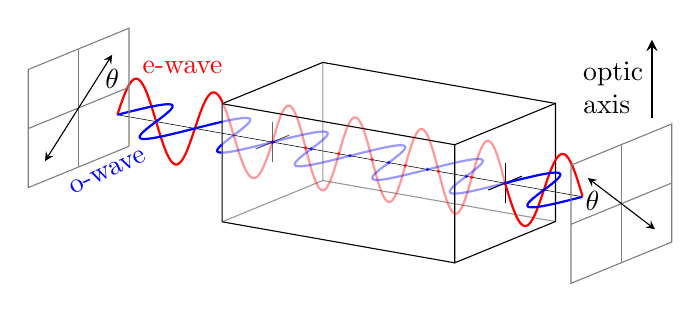
\begin{tikzpicture}[x={(-10:1)},y={(90:1)},z={(210:1)}]
        %\draw[step=1, gray,very thin] (-3,-3) grid (4,4);

        % Axes
        \draw[>=stealth, very thin] (-2,0,0) node[above] {} -- (4,0,0);
        %\draw[<->, >=stealth] (0,0,0) -- (0,2,0) node[above] {$y$};
        %\draw[<->, >=stealth] (0,0,0) -- (0,0,-2) node[left] {$x$};
        
        % plate endcaps
        % back
        \draw[] (0,0.75,-0.75) -- (0,0.75,0.75) -- (0,-0.75,0.75);
        \draw[opacity = 0.4] (0,0.75,-0.75) -- (0,-0.75,-0.75) -- (0,-0.75,0.75);
        \draw[opacity = 0.4] (0,-0.75,-0.75) -- (3,-0.75,-0.75);
        
        % cross
        \draw[opacity=0.6] (0,-0.25,0) -- (0,0.25,0);
        \draw[opacity=0.6] (0,0,-0.25) -- (0,0,0.25);
        
        % front
        \draw[] (3,-0.75,-0.75) -- (3,0.75,-0.75) -- (3,0.75,0.75) -- (3,-0.75,0.75) -- (3,-0.75,-0.75);
        
        % cross
        \draw[] (3,-0.25,0) -- (3,0.25,0);
        \draw[] (3,0,-0.25) -- (3,0,0.25);
        
        \draw[] (0,0.75,-0.75) -- (3,0.75,-0.75);
        \draw[] (0,0.75,0.75) -- (3,0.75,0.75);
        \draw[] (0,-0.75,0.75) -- (3,-0.75,0.75);
        
        % Waves    
        % region 1 (some parts hidden)
        \draw[red,thick] plot[domain=-2:-0.64,samples=200] (\x,{0.5*cos(deg(2*pi*\x-pi/2))},0);
        \draw[red,thick, opacity = 0.4] plot[domain=-0.64:0,samples=200] (\x,{0.5*cos(deg(2*pi*\x-pi/2))},0);
    
        \draw[blue,thick] plot[domain=-2:-0.9,samples=200] (\x,0,-{0.5*cos(deg(2*pi*\x-pi/2))});
        \draw[blue,thick, opacity = 0.4] plot[domain=-0.9:-0.4,samples=200] (\x,0,-{0.5*cos(deg(2*pi*\x-pi/2))});
        \draw[blue,thick] plot[domain=-0.4:-0.23,samples=200] (\x,0,-{0.5*cos(deg(2*pi*\x-pi/2))});
        \draw[blue,thick, opacity = 0.4] plot[domain=-0.23:0,samples=200] (\x,0,-{0.5*cos(deg(2*pi*\x-pi/2))});
        
        % region 2
        \draw[red,thick, opacity = 0.4] plot[domain=0:3,samples=200] (\x,{0.5*cos(deg(2*pi*\x + 1.05*\x - pi/2))},0);
        \draw[blue,thick, opacity = 0.4] plot[domain=0:3,samples=200] (\x,0,-{0.5*cos(deg(2*pi*\x - pi/2))});
        
        % region 3
        \draw[red,thick] plot[domain=3:4,samples=200] (\x,{0.5*cos(deg(2*pi*\x+pi/2))},0);
        \draw[blue,thick] plot[domain=3:4,samples=200] (\x,0,-{0.5*cos(deg(2*pi*\x-pi/2))});
        
        \foreach \n in {0,1,2,...,7}{
            \node at ({0.428*\n},0,0) [red, opacity = 0.7, circle,fill,inner sep=0.5]{};
        }
                \foreach \n in {0,1,2,...,6}{
            \node at ({0.5*\n},0,0) [blue, opacity = 0.7, circle,fill,inner sep=0.5]{};
        }
        
        % polarization planes
        \draw[gray] (-2.5,-0.75,-0.75) -- (-2.5,-0.75,0.75) -- (-2.5,0.75,0.75) -- (-2.5,0.75,-0.75) -- (-2.5,-0.75,-0.75);
        \draw[gray] (-2.5, 0, -0.75) -- (-2.5, 0, 0.75);
        \draw[gray] (-2.5, -0.75, 0) -- (-2.5, 0.75, 0);
        \draw[<->, >=stealth, thin] (-2.5,-0.5,0.5) -- (-2.5,0.5,-0.5);
        \node at (-2.5, 0.2, -0.5) {$\theta$};
        
        \draw[gray] (4.5,-0.75,-0.75) -- (4.5,-0.75,0.75) -- (4.5,0.75,0.75) -- (4.5,0.75,-0.75) -- (4.5,-0.75,-0.75);
        \draw[gray] (4.5, 0, -0.75) -- (4.5, 0, 0.75);
        \draw[gray] (4.5, -0.75, 0) -- (4.5, 0.75, 0);
        \draw[<->, >=stealth, thin] (4.5,-0.5,-0.5) -- (4.5,0.5,0.5);
        \node at (4.3, 0.07, 0.2) {$\theta$};
        
        \node at (-0.9, 0.9, 0.3) [red] {e-wave};
        \node at (-1.0, -0.1, 1.3) [blue, rotate=25] {o-wave};
        
        \draw[->, >=stealth, thick] (5.5,1.5,0.7) -- (5.5,2.5,0.7);
        \node at (5,1.8,0.7) [align=left] {optic\\axis};
        
        % Arrows
        %\foreach \x in {-0.5,-0.3,...,4.4} {
          %\draw[-,help lines] (\x,0,0) -- (\x,{cos(deg(pi*\x))},0);
          %\draw[-,help lines] (\x,0,0) -- (\x,0,-{cos(deg(pi*\x))});
        %}
        
        \Dimline[(0,1,-0.75)][(2,1,-0.75)][(3,1,-0.75)][d];
        
    \end{tikzpicture}
\end{document}